% This is a sample LaTeX file for a JOTA paper. A sample figure file (Fig_1.pdf) is required to typeset this file.
%A standard way of writing LaTeX files is to give everything a label: sections, formulas, figures, references, etc. Labeling makes it easy to modify a LaTeX file, but it is often difficult to create and remember the labels. Labeling is not used in this example.

\documentclass[smallextended,referee,envcountsect,]{svjour3}
% The option smallextended is the standard JOTA format.
% The option referee  makes the paper double-spaced.
% The option envcountsect numbers theorems, etc, by section.
% svjour3 is the document class for Springer journals.
\smartqed
%This command right justifies \qed throughout the paper.
\usepackage{graphicx}
\usepackage{amsmath}
%This package is used to insert figures.
\journalname{JOTA}

\begin{document}

\title{TESTE KOKALUKIA}

\subtitle{Using  the  LaTex Template}

\author{Tam\'as Terlaky}

\institute{Tam\'as Terlaky \at
             Lehigh University \\
              Bethlehem, PA 18015, USA\\
              terlaky@Lehigh.edu
           \and
              Virtual Author,  Corresponding author  \at
              University of Dreamland \\
              Dreamland\\
              author2@example.com
}

\date{Received: date / Accepted: date}
%The correct dates will be entered by the editor.

\maketitle

\begin{abstract}
Each submission must include an abstract, usually between 50 to 200 words. The abstract should give a clear and concise idea of the  content of the paper,  without the use of mathematical formulas, equations, and acronyms.
\end{abstract}
\keywords{Titles \and Sections \and Formulas \and More}
\subclass{49J53 \and  49K99 \and more}

%All acknowledgements should be placed in the back of the paper after Conclusions..

\section{Introduction}

The Introduction should contain a summary of the literature that pertains to the paper and a summary of the contents of the paper, as much as possible without formulas. It should spell out what is the novel contribution of the paper.  In the section References, the references should be listed in alphabetical order. Then, references should be cited in the text by the reference number in square brackets, for example, \cite{Huang} or \cite{Huang,Miele} or 
\cite{Huang,Miele,Nocedal,Ralston,Yang}.

\section{Statement of Purpose}

This journal publishes carefully selected papers covering mathematical optimization (and related topics) and its application to science and engineering. For a theoretical paper, the analytic treatment is compulsory. For an applications paper, the paper should be as much about a sophisticated application of an optimization method as it is about the solution of a particular problem. Therefore, an applications paper should contain a formal statement of the optimization problem in which the optimization variables, the objective function, and the constraints are clearly identified. If the paper is numerical in nature, the development and application of the numerical method should be discussed. Papers that present the formulation of a very large complex optimization problem with little discussion of optimization will probably be returned to the author with a recommendation to publish it in a journal more specifically related to the problem. It would be better for an author to select the simplest problem that is contained in the complex problem and to present it with its novel solution methodology.

\section{Prediction Equation}

\begin{equation}
   \dot{x}(t) = A_{\sigma(t)} + b_{\sigma(t)}
\end{equation}

lets use an augmented state 

\begin{align}
   \chi 
      &= \left[ \begin{matrix} x(t) \\ 1 \end{matrix} \right]
      \\
   \dot{\chi}(t) 
      &= \left[ \begin{matrix} \dot{x}(t) \\ \frac{\partial}{\partial t}(1) \end{matrix} \right] 
      = \left[ \begin{matrix} A x(t) = b_{\sigma(t)} \\ 0 \end{matrix} \right] 
      \\
   \dot{\chi}(t) 
      &= \underbrace{ \left[ \begin{matrix} A_{\sigma(t)} & b_{\sigma(t)} \\ 0 & 0 \end{matrix} \right] }_{\tilde{A}_{\sigma(t)}} \left[ \begin{matrix} x(t) \\ 1 \end{matrix} \right]
\end{align}

dynamic equation with augmented states

\begin{equation}
   \chi(t) = \tilde{A}_{\sigma(t)} \chi(t)
\end{equation}

\begin{equation}
   \chi(t_N) = 
      e^{\tilde{A}_{N-1} \Delta t_N}
      e^{\tilde{A}_{N-2} \Delta t_{N-1}}
      \dotsm
      e^{\tilde{A}_{0} \Delta t_{1}}
      \chi(t_0)
\end{equation}

let make 

\begin{equation}
   F_{i+1} = \tilde{A}\sigma(t_i)
\end{equation}

so

\begin{equation}
   \label{eq_augstate_1}
   \chi(t_N) = 
      e^{F_N \Delta t_N}
      e^{F_{N-1} \Delta t_{N-1}}
      \dotsm
      e^{F_{1} \Delta t_{1}}
      \chi(t_0)
\end{equation}

which also results in 

\begin{equation}
   \label{eq_augstate_2}
   \tilde{\chi}(t_N) = 
      e^{F_N \Delta \bar{t}_N}
      e^{F_{N-1} \Delta \bar{t}_{N-1}}
      \dotsm
      e^{F_{1} \Delta \bar{t}_{1}}
      \bar{\chi}(t_0)
\end{equation}

computing the error between the equations \eqref{eq_augstate_1} and \eqref{eq_augstate_2}

\begin{equation}
   e(t) = \chi(t) - \bar{\chi}(t)
\end{equation}

\begin{align}
   e(t_N) 
      &= 
      e^{F_N \Delta t_N} e^{F_{N-1} \Delta t_{N-1}} \dotsm e^{F_{1} \Delta t_{1}} \chi(t_0) - \\
      & \quad e^{F_N \Delta \bar{t}_N} e^{F_{N-1} \Delta \bar{t}_{N-1}} \dotsm e^{F_{1} \Delta \bar{t}_{1}} \chi(t_0) \\
      &= 
      e^{F_N (\Delta \bar{t}_N + \delta t_N)} e^{F_{N-1} (\Delta \bar{t}_{N-1} + \delta t_{N-1})} \dotsm e^{F_{1} (\Delta \bar{t}_{1} + \delta t_{1})} (\bar{\chi}(t_0) + e(t_0)) - \\
      & \quad e^{F_N \Delta \bar{t}_N} e^{F_{N-1} \Delta \bar{t}_{N-1}} \dotsm e^{F_{1} \Delta \bar{t}_{1}} \chi(t_0)
\end{align}



\section{Submission of a Paper}

Authors must submit their manuscripts online.  You can start by selecting "Submit Online" on the journal webpage at

www.springer.com/mathematics/journal/10957.

An Associate Editor  (AE) may be suggested, although the final selection of the AE will be made by the Editors. Also, please suggest several prospective reviewers, indicating title, full affiliation, and e-mail address.

Authors may request to exclude certain individuals to review their paper. Anu such request should be spelled out in the cover letter.

\subsection{Language}

 For both editorial considerations and final publication, English is the official language of the journal. Papers not written in correct English will be returned to the author before the review process is initiated. In organizations where English is not the operating language, access to an English editing service is often available.

\subsection{General Format}

 Manuscripts should be single spaced, with 12pts font size and all the pages numbered.  Figures and tables should be included in the text.  Papers should be limited to approximately 20 pages,  including figures and tables. This corresponds to approximately 18 journal pages.

\section{Editorial Procedure}

Authors are expected to comply with the overall style adopted for the journal. While it is impossible to cover every conceivable situation, the following instructions are provided for preparing a paper for publication.  The posted "Submission Guidelines" for authors should be followed. When in doubt, authors are advised to consult recent issues of the journal. Papers that do not comply with these instructions will be returned to the author.


\section{Sections and Statements}

Sections. The paper should contain at least 3 to 4 major sections. The first section is the Introduction. It should contain a summary of the literature that pertains to the paper and a summary of the contents of the paper, as much as possible without formulas. The last section is the Conclusions. It should contain short comments about the results (without formulas) but not like a second abstract.

Statements.  There are many statements used in the writing of a theoretical paper on optimization, such as definitions, assumptions,  remarks,  lemmas, propositions, theorems, and corollaries. While the format for each of these statements is different, LaTeX will use the correct format for each statement.  Each of these statements is numbered by major section. For example,  Theorem 3.1 denotes the first theorem of Section 3. Theorem 3.2 denotes the second theorem of Section 3, and so on.

The LaTeX commands for two theorems produce the following text:

\begin{theorem}
Type the first theorem of this section here.
\end{theorem}
{\it Proof}  The proof of the first theorem goes here.
\qed
\begin{theorem}
Type the second theorem of this section here.
\end{theorem}
{\it Proof}  The proof of the second theorem goes here.
\qed

For  other statements, use the same style that applies to theorems, that is, to present a proposition, replace theorem by proposition.  For statements that do not require a proof, omit the ``Proof" and ``qed" commands.


\section{Symbols, Equations, Figures, and Tables}

{\bf Symbols} Please use standard mathematical notation for  symbols, that is, Italic for single letters that denote mathematical constants, variables, and unknown quantities and Roman/upright for numerals, operators, and punctuation, and commonly defined functions or abbreviations, e.g., cos, det, e or exp, lim, log, max, min, sin, tan, d (for derivative). In the definition of a set, use IR for the set of reals, conv for convex hull, cl for closure, {A: B} for the set of A such that B holds, and double parallel arrows for set-valued maps.  Other symbols include  := for equality by definition and   an empty square at the right margin to denote the end of a proof. Please limit the use of acronyms.

{\bf Equations} Complexity of notation should be avoided, if possible. In particular, authors should avoid the simultaneous use of too many subscripts and superscripts. The LaTeX commands for one equation produce the following text:
\begin{equation}
a^2+b^2=c^2 .
\end{equation}
Equations should be cited in the text by the equation number in parentheses. In the text, avoid breaking an equation at the right-hand margin.

{\bf Figures and Tables}  Figures and Tables  should be provided in electronic form and included in the text. They should be placed in the text  after they are referenced.

The LaTeX commands for a single-column figure produce the following result:
% For one-column wide figures use
\begin{figure}[ht]
\begin{center}
% Use the relevant command to insert your figure file.
% For example, with the graphicx package use
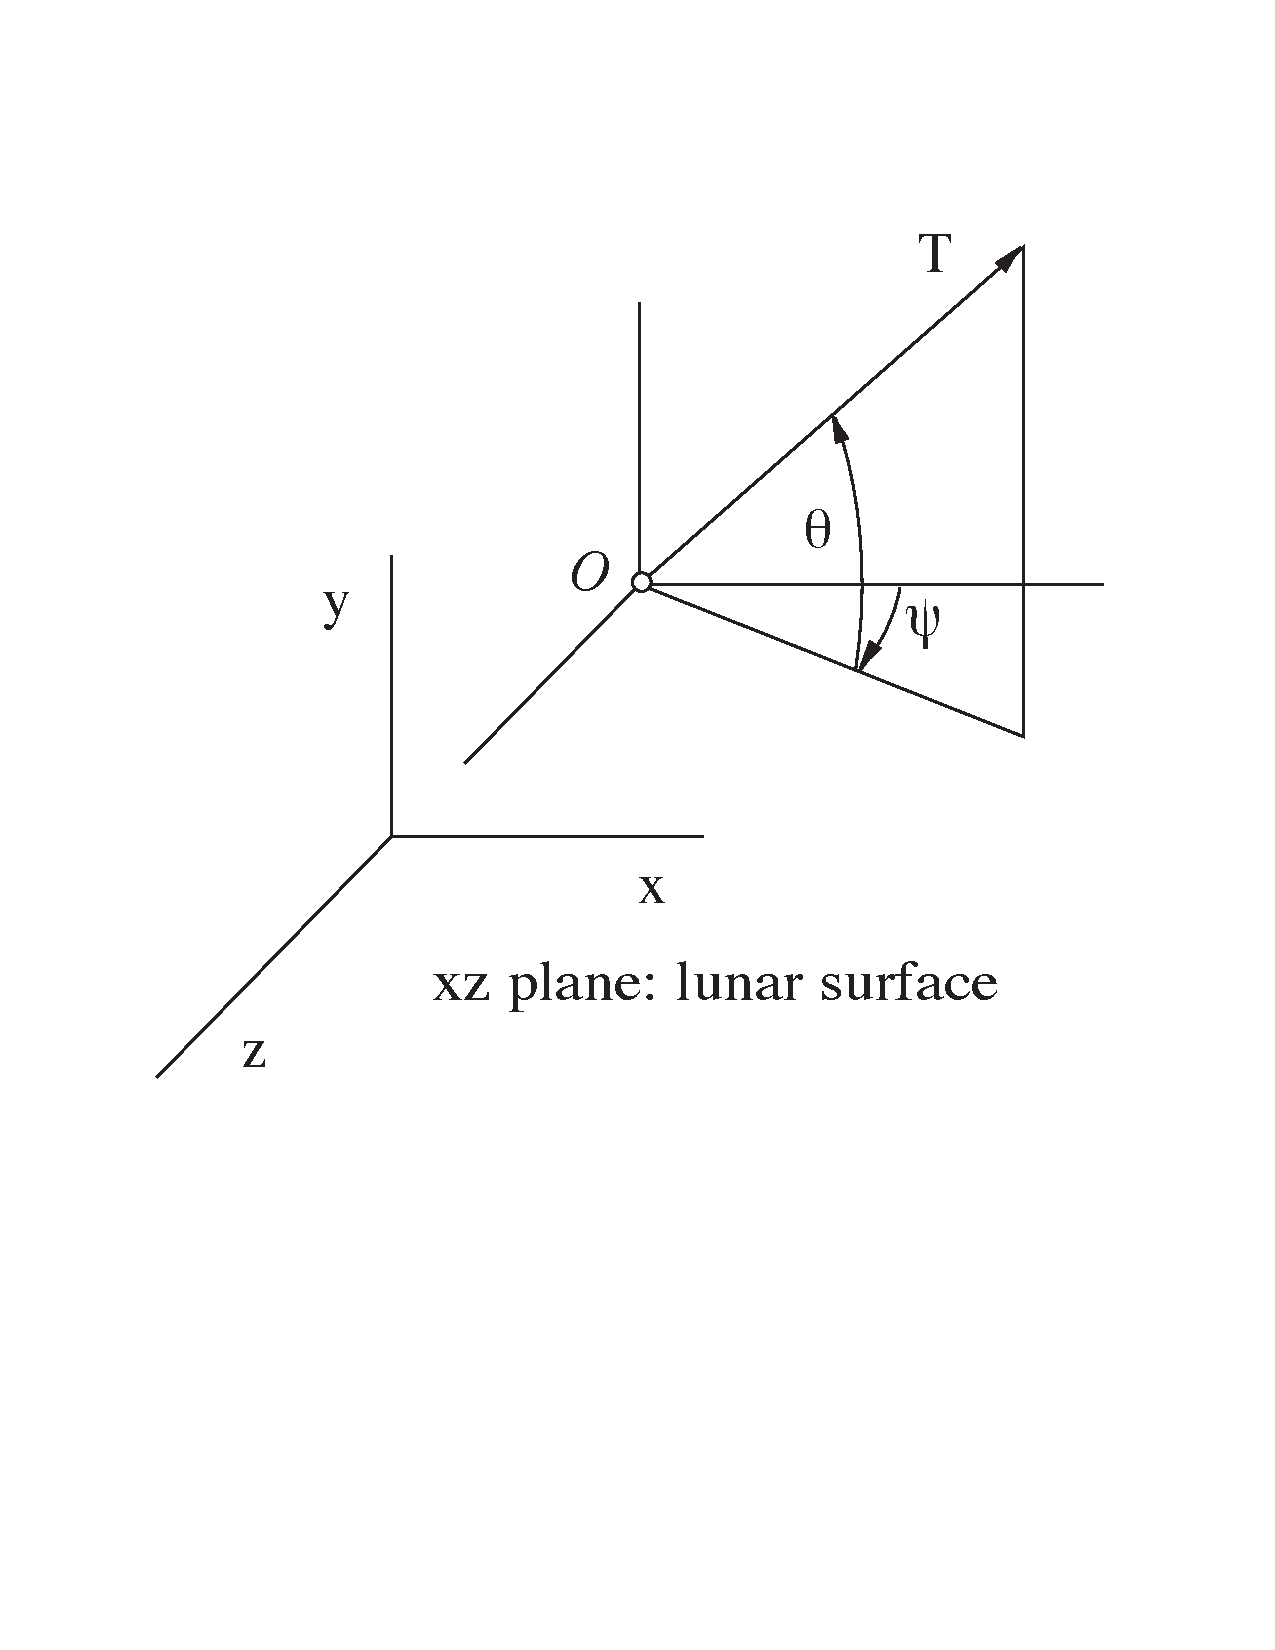
\includegraphics[width=2.0 in]{Fig_1.pdf}
% The figure caption is below the figure.
\end{center}
\vspace{-1 in}
\caption{Figures should be provided in electronic form and included in the text. }
\end{figure}

The LaTeX commands for a simple table produce the following result:
% For a simple table use
\begin{table}[ht]
% The table caption is above the table.
\caption{Tables should be provided in electronic form and included in the text. }
\vspace{.1 in}
\begin{center}
\begin{tabular}{|c|c|c|}
\hline
first & second & third  \\
\hline
number & number & number \\
number & number & number \\
\hline
\end{tabular}
\end{center}
\end{table}


\section{Conclusions}


This section is a summary of the major results of the paper, without formulas.

\begin{acknowledgements}
Acknowledgements to sponsoring agencies and individuals should be placed here.
\end{acknowledgements}

\appendix  %This command ends the counting of sections.
\section*{Appendix:  Instructions for Appendices}
If there is only one appendix, the title is Appendix. If there are appendices, the titles are Appendix A, Appendix B, and so on. Appendices should be referenced in the text. The numbering of equations,  figures, and tables should continue from the  text. For example,
\begin{equation}
a=b
\end{equation}
JOTA does not  accept electronic Supplementary Material.

%References
\begin{thebibliography}{plain}

% References must be listed in alphabetical order.

% Format for journal articles
\bibitem{Huang} Huang, H.Y.: Unified approach to quadratically convergent algorithms for function minimization. J. Optim. Theory Appl. 5, 354-405 (2009)

%Format for edited books
\bibitem{Miele} Miele, A. (ed.): Theory of Optimum Aerodynamic Shapes. Academic Press, New York (1965)


%Format for books
\bibitem{Nocedal}  Nocedal, J., Wright, S.J.: Numerical Optimization, Springer, New York  (2000)

%Format for articles in edited books
\bibitem{Ralston} Ralston, A.: Numerical integration methods for the solution of ordinary differential equations. In: Ralston, A., Wilf, H.S. (eds.): Mathematical Methods for Digital Computers, vol. 1, pp. 95-109. Wiley, New York (1960)

% Format for reports
\bibitem{Yang} Yang, T. L.: Optimal control for a rocket in a three-dimensional central force field. Technical Memorandum TM 69-2011-2, Bellcomm (1969)


\end{thebibliography}

\end{document}



%Old instruction:
%References
% BibTeX users  please use  \bibliographystyle{spmpsci_unsrt}. The option spmpsci_unsrt prints the references in old JOTA format  in the order they are cited.
%Otherwise, please use the following:





